\documentclass{beamer}

\usetheme{Pittsburgh}
\useinnertheme{default}
\setbeamertemplate{footline}[page number]
\setbeamertemplate{navigation symbols}{}

%\usepackage[utf8]{inputenc}
\usepackage{listings}
\lstset{ %
language=Ruby,                % choose the language of the code
basicstyle=\footnotesize,       % the size of the fonts that are used for the code
numbers=left,                   % where to put the line-numbers
numberstyle=\footnotesize,      % the size of the fonts that are used for the line-numbers
stepnumber=0,                   % the step between two line-numbers. If it's 1 each line 
                                % will be numbered
numbersep=5pt,                  % how far the line-numbers are from the code
backgroundcolor=\color{white},  % choose the background color. You must add \usepackage{color}
showspaces=false,               % show spaces adding particular underscores
showstringspaces=false,         % underline spaces within strings
showtabs=false,                 % show tabs within strings adding particular underscores
frame=none,	                % adds a frame around the code
tabsize=2,	                % sets default tabsize to 2 spaces
captionpos=b,                   % sets the caption-position to bottom
breaklines=true,                % sets automatic line breaking
breakatwhitespace=false,        % sets if automatic breaks should only happen at whitespace
title=\lstname,                 % show the filename of files included with \lstinputlisting;
                                % also try caption instead of title
escapeinside={\%*}{*)},         % if you want to add a comment within your code
emph={add,output,input,icecast,single,playlist,file,blank,sine,delay,amplify,sequence,in,out,
        clock,assign_new,oss,alsa,pulseaudio,mksafe,buffer,
              fallback,crossfade,http,fade,initial,final,cross},            % if you want to add more keywords to the set
keywordstyle=\color[rgb]{0,0.5,0.3},
emphstyle=\color{red},
stringstyle=\color{blue},
}

\newcommand{\kw}[1]{{\color{red} #1}}

\usepackage{tikz}
\usepackage[all]{xy}

\renewcommand{\emph}[1]{\alert{#1}}
\renewcommand{\textbf}[1]{{\color{blue} #1}}

%\newtheorem{lemme}{Lemme}
%\newtheorem{theorem}{Theorem}
\newtheorem{proposition}{Proposition}
%\theoremstyle{definition}
%\newtheorem{definition}{Definition}

% \author{David Baelde for Savonet}
\title{\emph{\LARGE Liquidsoap} \\
  A Programming Language for \\ Multimedia Streaming}
\date{David Baelde, Samuel Mimram, Romain Beauxis \\ and others}

\begin{document}

\begin{frame}
  \maketitle
\end{frame}

%% == INTRO ==================================

\begin{frame}{Liquidsoap}

  In 2003, an audio stream generator for Internet radio
  \[
  \xymatrix{
    *+[F]{\text{\textbf{source client}}}\ar[r]&
    *+[F]{\text{broadcast server}}
    \ar[r]\ar[dr]&
    *+{\text{listener}}\\
    &&*+{\text{listener}}
  }
  \]

  \begin{block}{A toolkit for multimedia streaming}
  \begin{itemize}
  \item Widely and variously used \\
     \quad music stations, news, DJ stations, \\
     \quad meta-radios, number stations, artistic experiments
  \item A programming \emph{language} for streaming
  \end{itemize}
  \end{block}

\end{frame}

\begin{frame}{Recipe}

\begin{block}{Liquidsoap}
\begin{enumerate}
\item<3-> A script language
\item<2-> A notion of {\em source} (interactive stream generator)
\item<1-> Interfaces: libraries, external and remote applications
\end{enumerate}
\end{block}

\uncover<4>{
\begin{block}{Language design}
\begin{itemize}
\item Users should have maximum access to the model
\item The language should prevent mistakes, hide complexity
\end{itemize}
\end{block}
}

\end{frame}

%% == MODELE =================================

\begin{frame}[fragile]{Principle}

% TODO this examples is fallible... fix it, say it?

\vspace{0.5cm}

\[
\xymatrix{
  *+[F]{\mathtt{input.http}} \ar[r] &
     *+[F]{\mathtt{fallback}} \ar[r]\ar[dr] &
     *+<7pt>[F=]{\mathtt{output.icecast}} \\
  *+[F]{\mathtt{playlist}}\ar[ur] &
     % *+[F]{\mathtt{crossfade}}\ar[u]
     &
     *+<7pt>[F=]{\mathtt{output.file}}\\
}
\]

\vspace{1cm}

\only<1>{\begin{block}{What is a source}
  \begin{itemize}
    \item Stream of samples, metadata, notion of track
    \item May be temporarily unavailable
    \item Passive (lazy) or active (typically, outputs)
  \end{itemize}
\end{block}}

\pause

\begin{block}{Script}
\begin{lstlisting}
live = input.http("http://server:8000/live.ogg")
music = playlist("/path/to/music")
s = fallback(track_sensitive=false,[live,music])
output.icecast(%vorbis,mount="radio.ogg",s)
output.file(%mp3(bitrate=16),"/path/to/backup.ogg",s)
\end{lstlisting}
\end{block}

\end{frame}

%% ===========================================

\begin{frame}{Clocks}

\[
\xymatrix{
  \text{\only<2->{\color{red}}remote server A} \ar[dr] &
        & \mbox{\only<2->{\color{gray}}remote server B} \\
  \text{\only<2->{\color{blue}}soundcard 1} \ar[r]      &
                \text{liquidsoap} \ar[ur]\ar[r]\ar[dr]
        & \mbox{\only<2->{\color{blue}}soundcard 1}     \\
  \text{\only<2->{\color{green}}soundcard 2} \ar[ur] &
        & \mbox{\only<2->{\color{blue}}backup file}
}
\]

\vfill
\pause
\pause

\begin{itemize}
\item Active sources are controlled by clocks
\item A liquidsoap instance may involve several clocks 
\item Each source belongs to a single clock
\end{itemize}

\end{frame}

\begin{frame}[fragile]{Clocks}

\[ \small
\xymatrix{
   *+[F]{\mathtt{playlist}}\ar[r]
   {\save "1,1"*+<10pt>[F--]\frm{} \restore}
   & *+[F]{\mathtt{crossfade}}\ar[r] &
      *+[F]{\mathtt{fallback}}\ar[r]& *+[F]{\mathtt{output}} \\
   & & *+[F]{\mathtt{jingles}}\ar[u]
   {\save "2,3"-<20pt>."1,4"."1,1"*+<20pt>[F--]\frm{} \restore}
   &
}
\]

\vfill

\begin{block}{Script}
\begin{lstlisting}
output.icecast(%vorbis,mount="myradio",
  fallback([crossfade(playlist("some.txt")),jingles]))
\end{lstlisting}
\end{block}

\end{frame}

\begin{frame}[fragile]{Clock uses}

\begin{block}{Avoid internal time inconsistencies}
\quad Cross-fading, stretching, \ldots
\end{block}

\vfill

\begin{block}{Deal with external time distortions}
\begin{lstlisting}
  input = input.oss()
  clock.assign_new(id="icecast",
    [output.icecast(%mp3,mount="blah",
                    mksafe(buffer(input)))])
  output.file(
    %mp3,"record-%Y-%m-%d-%H-%M-%S.mp3",
    input)
\end{lstlisting}
\end{block}

\end{frame}

%% ===========================================

\begin{frame}{Transitions}

  \begin{block}{When}
  \begin{itemize}
  \item Between tracks of the same source
  \item When switching from one source to another
  \end{itemize}
  \end{block}

  \begin{block}{What}
  \quad None, fade, cross-fade, insert jingle, \\
  \quad\quad adjust depending on volume, etc.
  \end{block}

  \vfill
  \pause

  \begin{block}{Generic solution}
\emph{
  \begin{center}
    transition =
     $\mathtt{source} \times \mathtt{source} \rightarrow \mathtt{source}$.
  \end{center}
}
  \end{block}

\end{frame}

\begin{frame}{Cross-fading}

\begin{itemize}
\item \lstinline{s = fade.out(duration=3., s)}
\only<1>{
  \begin{center}
  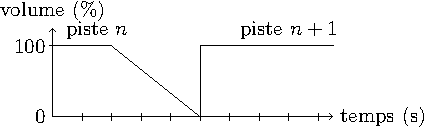
\includegraphics{transitions-out.pdf}
  \end{center}
}
\item<2-> \lstinline{s = fade.in(duration=2., s)}
\only<2>{
  \begin{center}
  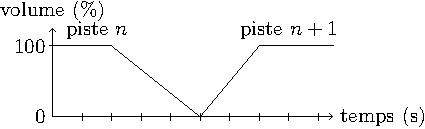
\includegraphics{transitions-out-in.pdf}
  \end{center}
}
\item<3> \lstinline{cross(duration=2., (fun (a,b) -> add([a,b])), s)}
\only<3>{
  \begin{center}
  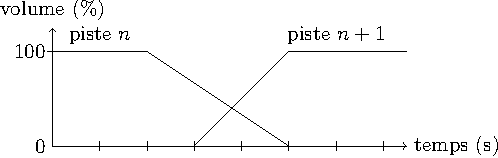
\includegraphics{transitions.pdf}
  \end{center}
}
\end{itemize}

\end{frame}

\begin{frame}[fragile]{Demo: smooth add}

\vspace{0.3cm}

\begin{lstlisting}
def smooth_add(~delay=0.5,~p=0.2,~normal,~special)
  fade.final = fade.final(duration=delay*2.)
  fade.initial = fade.initial(duration=delay*2.)
  fallback(track_sensitive=false,
    [special,normal],
    transitions=[
      fun(normal,special)->
        add(normalize=false,
            [amplify(p,normal),
             amplify(1.-p,fade.final(normal)),
             sequence([blank(duration=delay),
                       amplify(1.-p,special)])]),
      fun(special,normal)->
        add(normalize=false,
            [amplify(p,normal),
             amplify(1.-p,fade.initial(normal))])
    ])
end
\end{lstlisting}

%% ./src/liquidsoap scripts/utils.liq 'output.pulseaudio(visu.volume(smooth_add(special=delay(3.,blank(duration=4.)),normal=sine(330.))))'

\end{frame}

%% ===========================================

\begin{frame}{Features}

\begin{block}{Elementary sources}
\begin{itemize}
\item File, playlist, queue, dynamically chosen file
\end{itemize}
\end{block}

\begin{block}{Source operators}
\begin{itemize}
\item Stream processing: filters, effects, analysis
\item Metadata processing: inserting, modifying, dropping
\item Control: switching, mixing, sequencing
\item Transitions: switch, cross, smart cross
\item Event handlers: tracks, metadata, blank
\end{itemize}
\end{block}

\end{frame}

\begin{frame}{Features}

\begin{block}{Interfaces}
\begin{itemize}
\item Icecast, Shoutcast and compatible: output, relay and host
\item ALSA, OSS, Jack, Pulseaudio, AO\ldots
\end{itemize}
\end{block}

\begin{block}{Files}
\begin{itemize}
\item Most formats (WAV, Vorbis, MP3, AAC+, Flac, external\ldots)
\item Request, resolution (HTTP, speech, custom protocol)
\end{itemize}
\end{block}

\begin{block}{Server}
\begin{itemize}
\item Execute commands through TCP (telnet) or Unix stockets
\item Push, skip, monitor\ldots custom commands
\end{itemize}
\end{block}

\end{frame}

%% == LANGUAGE =================================

\begin{frame}[fragile]{Liquidsoap, the language}

  \begin{block}{Why a new language}
  \begin{itemize}
    \item Functional, statically typed, labelled and optional arguments
\begin{center}\tiny\begin{verbatim}
$ liquidsoap -h cross
Generic cross operator, allowing the composition of the N last seconds of a track with
the beginning of the next track.
Type: (?id:string, ?duration:float, ?override:string, ?inhibit:float, ?minimum:float,
       ?conservative:bool, ?active:bool, ((source('a), source('a))->source('a)),
       source('a))->source('a)
Parameters:
* duration : float (default 5.)
    Duration in seconds of the crossed end of track. This value can be changed on a ...
* override : string (default "liq_start_next")
    Metadata field which, if present and containing a float, overrides the 'duration' ...
* inhibit : float (default -1.)
    Minimum delay between two transitions. It is useful in order to avoid that a ...
* minimum : float (default -1.)
    Minimum duration (in sec.) for a cross: If the track ends without any warning ...
* conservative : bool (default false)
    Do not trust remaining time estimations, always buffering data in advance. This ...
...
\end{verbatim}\end{center}
    \item Need to analyze scripts and functions
    \item Specific type system
    \item User-friendly doc and syntactic sugar
  \end{itemize}
  \end{block}

\end{frame}

\begin{frame}[fragile]{Type inference}

\emph{Automatically} infer types
\begin{verbatim}
  $ f = fun(x) -> x*2 ;;
  f : (int)->int = <fun>
\end{verbatim}

\vfill

Unconstrained types yield \emph{polymorphic} values
\begin{verbatim}
  $ g = fun(x,y) -> [x,y] ;;
  g : ('a,'a)->['a] = <fun>

  $ morning = fun(s)->switch([({7h-12h30},s)]) ;;
  morning : (source('a))->source('a) = <fun>
\end{verbatim}

\end{frame}

\begin{frame}[fragile]{Static types $\Rightarrow$ \emph{static} analysis}

\begin{lstlisting}
$ f("3");;
At line 1, char 3-5:
  this value has type
    string
  but it should be a subtype of
    int

$ g(blank(),blank) ;;
At line 1, char 16:
  this value has type
    (?id:_,?duration:_)->_
  but it should be a subtype of (the type of the value at line 1, char 12)
    source(_) (infered at line 1, char 8-9)

$ source = blanc() ;;
At line 1, char 15: the variable blanc used here
  has not been previously defined.
\end{lstlisting}

\end{frame}

\begin{frame}{Stream content}

\begin{block}{Each source has its own content type}
\quad Mono, stereo, video, video and audio, MIDI, etc. \\
\quad \emph{Arity}: $n$ (fixed) ou $\star + n$ (variable) with \emph{subtying} \\
 ~ \\
  \texttt{\small
    \begin{tabular}{rcl}
    swap&:&(source(2,0,0)) -> source(2,0,0)\\
    blank &:& () -> source('*a,'*b,'*c) \\
    on\_metadata&:&(handler,source('*a,'*b,'*c)) -> \\
           & & source('*a,'*b,'*c)\\
    echo&:&(delay:float,source('\#a,0,0)) -> \\
        & & source('\#a,0,0)\\
    % DB vire le prefixe "video." pour faire de la place a gauche
    %  en vrai greyscale veut du fixed arity, pcq son implem est pas
    %  assez générale
    greyscale&:&(source('*a,'*b+1,'*c)) -> \\ & & source('*a,'*b+1,'*c)\\
    output.file &:& 
       (format('*a,'*b,'*c), string, \\
     & & \phantom{(}source('*a,'*b,'*c)) ->\\
     & & source('*a,'*b,'*c)
    \end{tabular}
  }
\end{block}

\end{frame}

\begin{frame}[fragile]{Stream content}

\vfill

\textbf{Content is inferred}, usually from encoding formats
\begin{lstlisting}
$ output.file(%mp3,"/tmp/dump.mp3",
           input.http("http://blah"),fallible=true) ;;
 - : active_source(audio=2,video=0,midi=0)

$ output.file(%mp3(mono),"/tmp/dump.mp3",
           input.http("http://blah"),fallible=true) ;;
 - : active_source(audio=1,video=0,midi=0)
\end{lstlisting}

\vfill

Explicit conversions, \textbf{content-sensitive} decoding
\begin{lstlisting}
$ output.pulseaudio(
    audio_to_stereo(playlist("list.txt")),
    fallible=true) ;;
 - : active_source(audio=2,video=0,midi=0)
\end{lstlisting}

\end{frame}

%% ===========================================

% TODO high-level, safe / functional but impure /
% declarative, out of time, black box

\begin{frame}{Conclusion}

\begin{block}{Slogans}
\begin{itemize}
\item Programming language interfaces are almighty
\item Static languages not only for advanced programmers
\item Advanced features for the masses \\
\begin{flushright}
  {\small static types, inference, subtyping, polymorphism}
\end{flushright}
\end{itemize}
\end{block}

\vfill

\begin{block}{Future}
\begin{itemize}
\item Video and MIDI, interactive uses, community
\item More structured programming, OO-like
\item Get rid of \emph{black-box sources}, out-of-time programs
\item \emph{Compile} the language, efficient DSP
  % To name a few: chuck, puredata, faust, streamit \ldots
\end{itemize}
\end{block}

\end{frame}

\end{document}
